\documentclass[10pt]{article}
\usepackage[usenames]{color} %used for font color
\usepackage{amssymb} %maths
\usepackage{amsmath} %maths
\usepackage[utf8]{inputenc} %useful to type directly diacritic characters
\begin{document}
\begin{align*}\documentclass{tufte-handout}
\usepackage{graphicx}

\title{Conway's Game of Life}

\author[The Academy]{Ilya Michurin}

%\date{28 March 2010} % without \date command, current date is supplied

%\geometry{showframe} % display margins for debugging page layout

\usepackage{graphicx} % allow embedded images
  \setkeys{Gin}{width=\linewidth,totalheight=\textheight,keepaspectratio}
  \graphicspath{{graphics/}} % set of paths to search for images
\usepackage{amsmath}  % extended mathematics
\usepackage{booktabs} % book-quality tables
\usepackage{units}    % non-stacked fractions and better unit spacing
\usepackage{multicol} % multiple column layout facilities
\usepackage{lipsum}   % filler text
\usepackage{fancyvrb} % extended verbatim environments
  \fvset{fontsize=\normalsize}% default font size for fancy-verbatim environments
  
  
  
    %MADNESS
  
  \usepackage[T1]{fontenc} % Use 8-bit encoding that has 256 glyphs
\usepackage{fourier} % Use the Adobe Utopia font for the document - comment this line to return to the LaTeX default
\usepackage[english]{babel} % English language/hyphenation
\usepackage{amsmath,amsfonts,amsthm} % Math packages
\usepackage{mathtools}% http://ctan.org/pkg/mathtools
\usepackage{etoolbox}% http://ctan.org/pkg/etoolbox
\usepackage{lipsum} % Used for inserting dummy 'Lorem ipsum' text into the template
\usepackage{units}% To use \nicefrac
\usepackage{cancel}% To use \cancel
%\usepackage{physymb}%To use r
\usepackage{sectsty} % Allows customizing section commands
\usepackage[dvipsnames]{xcolor}
\usepackage{pgf,tikz}%To draw 
\usepackage{pgfplots}%To draw 
\usetikzlibrary{shapes,arrows}%To draw 
\usetikzlibrary{patterns,fadings}
 \usetikzlibrary{decorations.pathreplacing}%To draw curly braces 
 \usetikzlibrary{snakes}%To draw 
 \usetikzlibrary{spy}%To do zoom-in
 \usepackage{setspace}%Set margins and such
 %\usepackage{3dplot}%To draw in 3D
\usepackage{framed}%To get shade behind text



\definecolor{shadecolor}{rgb}{0.9,0.9,0.9}%setting shade color
\allsectionsfont{\centering \normalfont\scshape} % Make all sections centered, the default font and small caps

% Standardize command font styles and environments
\newcommand{\doccmd}[1]{\texttt{\textbackslash#1}}% command name -- adds backslash automatically
\newcommand{\docopt}[1]{\ensuremath{\langle}\textrm{\textit{#1}}\ensuremath{\rangle}}% optional command argument
\newcommand{\docarg}[1]{\textrm{\textit{#1}}}% (required) command argument
\newcommand{\docenv}[1]{\textsf{#1}}% environment name
\newcommand{\docpkg}[1]{\texttt{#1}}% package name
\newcommand{\doccls}[1]{\texttt{#1}}% document class name
\newcommand{\docclsopt}[1]{\texttt{#1}}% document class option name
\newenvironment{docspec}{\begin{quote}\noindent}{\end{quote}}% command specification environment
\begin{document}

\maketitle % Print the title section
\begin{marginfigure}%
 \includegraphics[width=\linewidth]{maxresdefault}
 \caption{This is an example of the Game of Life}
 \label{fig:marginfig}
\end{marginfigure}


\normalsize

\vspace{1cm}



\section{Main Menu - Program Code}
%this generates 1cm of vertical space
\vspace{1cm}





\vspace{1cm}


\large

\section{1) {\color{red}What is Conway's Game of Life}}

{\color{blue}Conway's Game of Life}, also known simply as {\color{blue}Life}, is a cellular automaton devised by the British mathematician {\color{blue}John Horton Conway} in 1970.

\begin{marginfigure}
  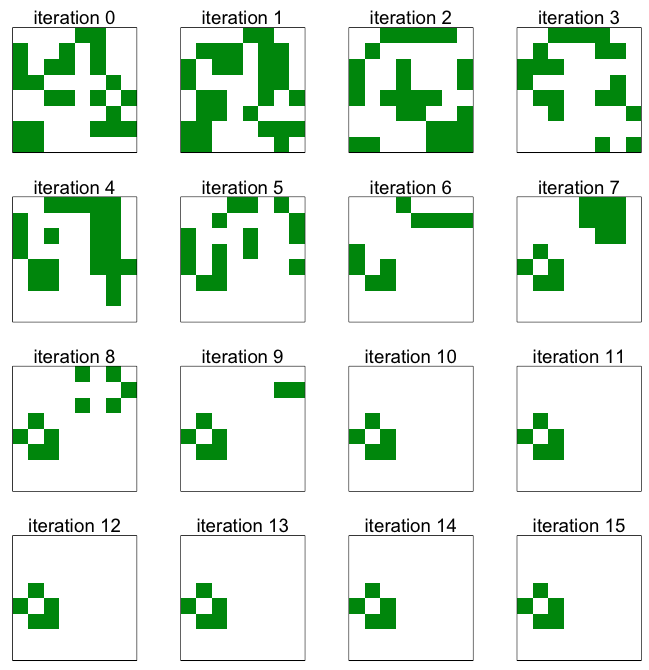
\includegraphics[width=\linewidth]{life-blog-image-2.png}
  \caption{In this picture 12 section are presented of the Game of Life, highlighted squares are the cells that live.}
  \label{fig:marginfig}
\end{marginfigure}

The "game" is a zero-player game, meaning that its evolution is determined by its initial state, requiring no further input. One interacts with the Game of Life by creating an initial configuration and observing how it evolves or, for advanced players, by creating patterns with particular properties.

\normalsize

\section{2) Python Code}


\marginnote[70pt]{\large{After reading a code and copying it into your PYTHON, please BE CAREFUL!!!! The reason is the grid number, put the most lucky number for your laptop/PC in the way not to burn it.     XD}}



\begin{framed}
\begin{verbatim}

import random
from graphics import *


def empty(N):
    a=[]
    for i in range(N):
        b=[]
        for j in range(N):
            b=b+[0]
        a=a+[b]
    return a
\end{verbatim}
\end{framed}

\marginnote[70pt]{\large{{\color{red}The number that you put will be your grid size, if you put 6 or 5, your grid will be 6x6 or 5x5, so pick the good one}}}







\marginnote[70pt]{\large{It all depends on a size, if you do not know settings of your computer, it will take more time to process the whole code, don't even try to enjoy the time of processing the grid of 20x20  }}

\begin{framed}
\begin{verbatim}

def fill(a,p):
    N=len(a)
    for i in range(N):
        for j in range(N):
            if random.uniform(0,1)<p:
                a[i][j]=1

def update(A,B):
    N=len(A)
    for i in range(N):
        for j in range(N):
            neigh=A[(i-1)%N][(j-1)%N]+A[(i-1)%N][j]+
            		     A[(i-1)%N][(j+1)%N]+A[i][(j-1)%N]+
			                  A[i][(j+1)%N]+A[(i+1)%N][(j-1)%N]+
			                  A[(i+1)%N][j]+A[(i+1)%N][(j+1)%N]
            if A[i][j]==0:
                if neigh==3:
                    B[i][j]=1
                else:
                    B[i][j]=0
            else:
                if neigh==2 or neigh==3:
                    B[i][j]=1
                else:
                    B[i][j]=0


def gen2Dgraphic(N):
    a=[]
    for i in range(N):
        b=[]
        for j in range(N):
            b=b+[Circle(Point(i,j),.49)]
        a=a+[b]
    return a

def push(B,A):
    N=len(A)
    for i in range(N):
        for j in range(N):
            A[i][j]=B[i][j]
            
def drawArray(A,a,window):
    N=len(A)
    for i in range(N):
        for j in range(N):
            if A[i][j]==1:
                a[i][j].undraw()
                a[i][j].draw(window)
            if A[i][j]==0:
                a[i][j].undraw()

N=int(input("Enter the grid dimension  "))
win = GraphWin()
win.setCoords(-1,-1,N+1,N+1)
grid=empty(N)
grid2=empty(N)
circles=gen2Dgraphic(N)
fill(grid,0.3)

while True:
    drawArray(grid,circles,win)
    update(grid,grid2)
    push(grid2,grid)

\end{verbatim}
\end{framed}

\marginnote[40pt]{\textbf{{\color{yellow}We showed you our version} of work that does not work properly, but it works. There is one problem that we could not how to solve the problem with putting changes of the new state in one window }}


\section{3) {\color{red}Rules of the Conway's Game of Life}}

The universe of the Game of Life is an infinite two-dimensional orthogonal grid of square cells, each of which is in one of two possible states, alive or dead. Every cell interacts with its eight neighbours, which are the cells that are horizontally, vertically, or diagonally adjacent. At each step in time, the following transitions occur:
	
	1)Any live cell with {\color{blue}two or three} live neighbours lives on to the next generation.

	2)Any dead cell with exactly three live neighbours becomes a live cell, as if by reproduction.
	
	3){\color{red}In any other situation cell dies}. 

\section{4) How our program does it's job

So, by the creating a first erray, we crate the "Old State" or "original" one where we put cell in random positions, after the creating, by the graph library, all lines and circles=cells, we started to create a new array, which is also random, and that will follow all the rules of Game of Life, after by using again graphics library, we get a ready "New State" of cells which applied all the rules.  
}


\bibliography{sample-handout}
\bibliographystyle{plainnat}


\begin{shaded}
\begin{verbatim}

As the result, we got 

continuous creation of "New States" which you can stop
only by killing the program 

Because we couldn't put changing of live cells 
in one state

\end{verbatim}
\end{shaded}



\vspace{1cm}






\end{document}\end{align*}
\end{document}